%% abtex2-modelo-trabalho-academico.tex, v-1.9.6 laurocesar
%% Copyright 2012-2016 by abnTeX2 group at http://www.abntex.net.br/ 
%% This work consists of the files abntex2-modelo-trabalho-academico.tex,
%% abntex2-modelo-include-comandos and abntex2-modelo-references.bib
%%

%% O abnTeX2, evolução do abnTeX (ABsurd Norms for TeX*), é uma suíte para LaTeX que atende os requisitos das normas da ABNT (Associação Brasileira de Normas Técnicas) para elaboração de documentos técnicos e científicos brasileiros, como artigos científicos, relatórios técnicos, trabalhos acadêmicos como teses, dissertações, projetos de pesquisa e outros documentos do gênero. A suíte abnTeX2 é composta por uma classe, por pacotes de citação e de formatação de estilos bibliográficos, por exemplos, modelos de documentos e por uma ampla documentação.
%%

\documentclass[
	% -- opções da classe memoir --
	12pt,				% tamanho da fonte
	openright,			% capítulos começam em pág ímpar (insere página vazia caso preciso)
	oneside,			% para impressão em recto e verso. Oposto a oneside
	a4paper,			% tamanho do papel. 
	% -- opções da classe abntex2 --
	%chapter=TITLE,		% títulos de capítulos convertidos em letras maiúsculas
	%section=TITLE,		% títulos de seções convertidos em letras maiúsculas
	%subsection=TITLE,	% títulos de subseções convertidos em letras maiúsculas
	%subsubsection=TITLE,% títulos de subsubseções convertidos em letras maiúsculas
	% -- opções do pacote babel --
	english,			% idioma adicional para hifenização
	french,				% idioma adicional para hifenização
	spanish,			% idioma adicional para hifenização
	brazil				% o último idioma é o principal do documento
	]{abntex2}

% ---
% Pacotes básicos 
% ---
\usepackage{lmodern}			% Usa a fonte Latin Modern	
\usepackage[T1]{fontenc}		% Selecao de fontes.
\usepackage[utf8]{inputenc}		% Codificacao do documento
\usepackage{lastpage}			% Ficha catalográfica
\usepackage{indentfirst}		% Indenta o 1 parágrafo.
\usepackage{color}				% Controle das cores
\usepackage{graphicx}			% Inclusão de gráficos
\usepackage{microtype} 			% melhorias de justificação
\usepackage[]{pdfpages}         %permite colocar pdf no texto
\usepackage{pdflscape}
\usepackage{adjustbox}
\usepackage{multirow}

\newcommand{\quadroname}{Quadro}
\newcommand{\listofquadrosname}{Lista de quadros}

\newfloat{quadro}{loq}{\quadroname}
\newlistof{listofquadros}{loq}{\listofquadrosname}
\newlistentry{quadro}{loq}{0}

% configurações para atender às regras da ABNT
\setfloatadjustment{quadro}{\centering}
\counterwithout{quadro}{chapter}
\renewcommand{\cftquadroname}{\quadroname\space} 
\renewcommand*{\cftquadroaftersnum}{\hfill--\hfill}

% Configuração de posicionamento padrão:
\setfloatlocations{quadro}{hbtp}

% Pacote para a definição de novas cores
\usepackage{xcolor}
% Definindo novas cores
\definecolor{verde}{rgb}{0.25,0.5,0.35}
\definecolor{jpurple}{rgb}{0.5,0,0.35}
\definecolor{darkgreen}{rgb}{0.0, 0.2, 0.13}
\usepackage[numberbychapter=false]{listings}

% Altera o nome padrão do rótulo usado no comando \autoref{}
\renewcommand{\lstlistingname}{Código}
% Altera o rótulo a ser usando no elemento pré-textual "Lista de código"
\renewcommand{\lstlistlistingname}{Lista de códigos}

% Configura a ``Lista de Códigos'' conforme as regras da ABNT (para abnTeX2)
\begingroup\makeatletter
\let\newcounter\@gobble\let\setcounter\@gobbletwo
  \globaldefs\@ne \let\c@loldepth\@ne
  \newlistof{listings}{lol}{\lstlistlistingname}
  \newlistentry{lstlisting}{lol}{0}
\endgroup

\renewcommand{\cftlstlistingaftersnum}{\hfill--\hfill}

\let\oldlstlistoflistings\lstlistoflistings
\renewcommand{\lstlistoflistings}{%
   \begingroup%
   \let\oldnumberline\numberline%
   \renewcommand{\numberline}{\lstlistingname\space\oldnumberline}%
   \oldlstlistoflistings%
   \endgroup}

\newcommand{\estiloCodigo}{
\lstset{
    language=Java,
    basicstyle=\ttfamily\small,
    keywordstyle=\color{blue}\bfseries,
    stringstyle=\color{orange},
    commentstyle=\color{black},
    morecomment=[s][\color{blue}]{/**}{*/},
    extendedchars=true,
    showspaces=false,
    showstringspaces=false,
    numbers=none,
    numberstyle=\tiny,
    breaklines=true,
    backgroundcolor=\color{cyan!3},
    breakautoindent=true,
    captionpos=b,
    xleftmargin=0pt,
    tabsize=1
}}


% ---
% Pacotes adicionais
% ---
\usepackage{lipsum}				% para geração de dummy text



% ---
% Pacotes de citações
% ---
\usepackage[brazilian,hyperpageref]{backref}	 % Paginas com as citações na bibl
\usepackage[alf]{abntex2cite}	% Citações padrão ABNT

% --- 
% CONFIGURAÇÕES DE PACOTES
% --- 

% ---
% Configurações do pacote backref
% Usado sem a opção hyperpageref de backref
\renewcommand{\backrefpagesname}{Citado na(s) página(s):~}
% Texto padrão antes do número das páginas
\renewcommand{\backref}{}
% Define os textos da citação
\renewcommand*{\backrefalt}[4]{
	\ifcase #1 %
		Nenhuma citação no texto.%
	\or
		Citado na página #2.%
	\else
		Citado #1 vezes nas páginas #2.%
	\fi}%
% ---

% ---
% Informações de dados para CAPA e FOLHA DE ROSTO
% ---
\titulo{Título do trabalho}
\autor{Roberta Santos Vieira}
\local{Araçuaí -- MG}
\data{2023}
\orientador{Prof. Felipe Túlio de Castro}
\coorientador{Prof. José Lucas Pereira Luiz}
\instituicao{%
  Instituto Federal de Educação, Ciência e Tecnologia do Norte de Minas Gerais -- IFNMG
  \par
  Tecnologia em Análise e Desenvolvimento de Sistemas
  \par
  Campus Araçuaí}
\tipotrabalho{Monografia (Graduação)}

% O preambulo deve conter o tipo do trabalho, o objetivo, 
% o nome da instituição e a área de concentração 

%PREAMBULO PARA AS MONOGRAFIAS (TCC II)
%\preambulo{Monografia apresentada ao curso de Análise e Desenvolvimento de Sistemas do Instituto Federal de Educação, Ciência e Tecnologia do Norte de Minas Gerais, Campus Araçuaí, como parte dos requisitos para obtenção do título de Tecnólogo em Análise e Desenvolvimento de Sistemas.}

%PREAMBULO PARA OS PROJETOS DE PESQUISA (TCC I)
\preambulo{Projeto de pesquisa apresentado ao curso de Análise e Desenvolvimento de Sistemas do Instituto Federal de Educação, Ciência e Tecnologia do Norte de Minas Gerais, Campus Araçuaí, como parte dos requisitos para aprovação na disciplina de TCC I.}
% ---


% ---
% Configurações de aparência do PDF final

% alterando o aspecto da cor azul
\definecolor{blue}{RGB}{41,5,195}

% informações do PDF
\makeatletter
\hypersetup{
     	%pagebackref=true,
		pdftitle={\@title}, 
		pdfauthor={\@author},
    	pdfsubject={\imprimirpreambulo},
	    pdfcreator={LaTeX with abnTeX2},
		pdfkeywords={abnt}{latex}{abntex}{abntex2}{trabalho acadêmico}, 
		colorlinks=true,       		% false: boxed links; true: colored links
    	linkcolor=black,          	% color of internal links
    	citecolor=black,        		% color of links to bibliography
    	filecolor=magenta,      		% color of file links
		urlcolor=blue,
		bookmarksdepth=4
}
\makeatother
% --- 

% --- 
% Espaçamentos entre linhas e parágrafos 
% --- 

% O tamanho do parágrafo é dado por:
\setlength{\parindent}{1.3cm}

% Controle do espaçamento entre um parágrafo e outro:
\setlength{\parskip}{0.2cm}  % tente também \onelineskip

% ---
% compila o indice
% ---
\makeindex
% ---

% ----
% Início do documento
% ----
\begin{document}

% Seleciona o idioma do documento (conforme pacotes do babel)
%\selectlanguage{english}
\selectlanguage{brazil}

% Retira espaço extra obsoleto entre as frases.
\frenchspacing 

% ----------------------------------------------------------
% ELEMENTOS PRÉ-TEXTUAIS
% ----------------------------------------------------------

% ---
% Capa
% ---
\imprimircapa
% ---

% ---
% Folha de rosto (* indica que haverá ficha bibliográfica)
% ---
\imprimirfolhaderosto*
% ---

% ---
% Ficha Catalográfica
% ---

% Isto é um exemplo de Ficha Catalográfica, ou ``Dados internacionais de catalogação-na-publicação''. Você pode utilizar este modelo como referência. Porém, provavelmente a biblioteca da sua universidade lhe fornecerá um PDF com a ficha catalográfica definitiva após a defesa do trabalho. Quando estiver com o documento, salve-o como PDF no diretório do seu projeto e substitua todo o conteúdo de implementação deste arquivo pelo comando abaixo:

% \begin{fichacatalografica}
%     \includepdf{fig_ficha_catalografica.pdf}
% \end{fichacatalografica}

\begin{fichacatalografica}
	\sffamily
	\vspace*{\fill}					% Posição vertical
	\begin{center}					% Minipage Centralizado
	\fbox{\begin{minipage}[c][8cm]{13.5cm}		% Largura
	\small
	\imprimirautor
	%Sobrenome, Nome do autor
	
	\hspace{0.5cm} \imprimirtitulo  / \imprimirautor. --
	\imprimirlocal, \imprimirdata 
	
	\hspace{0.5cm} \pageref{LastPage} p. : il. (algumas color.).\\
	
	\hspace{0.5cm} \imprimirorientadorRotulo~\imprimirorientador\\
	
	\hspace{0.5cm}
	\parbox[t]{12.5cm}{\textwidth}{\imprimirtipotrabalho~--~\imprimirinstituicao,
	\imprimirdata.}\\
	
	\hspace{0.5cm}
		1. Palavra-chave1.
		2. Palavra-chave2.
		2. Palavra-chave3.
		I. \imprimirorientador.
		II. Instituto Federal de Educação, Ciência e Tecnologia do Norte de Minas Gerais.
		III. Núcleo de Informática.
		IV. \imprimirtitulo 			
	\end{minipage}}
	\end{center}
\end{fichacatalografica}

% ---
% Folha de aprovação
% ---

% Isto é um exemplo de Folha de aprovação, elemento obrigatório da NBR 14724/2011 (seção 4.2.1.3). Você pode utilizar este modelo até a aprovação do trabalho. Após isso, substitua todo o conteúdo deste arquivo por uma imagem da página assinada pela banca com o comando abaixo:
% \includepdf{folhadeaprovacao_final.pdf}
\begin{folhadeaprovacao}

  \begin{center}
    {\ABNTEXchapterfont\large\imprimirautor}

    \vspace*{\fill}\vspace*{\fill}
    \begin{center}
      \ABNTEXchapterfont\bfseries\Large\imprimirtitulo
    \end{center}
    \vspace*{\fill}
    
    \hspace{.45\textwidth}
    \begin{minipage}{.5\textwidth}
        \imprimirpreambulo
    \end{minipage}%
    \vspace*{\fill}
   \end{center}
        
   Trabalho aprovado. \imprimirlocal, 06 de fevereiro de 2024:

   \assinatura{\textbf{\imprimirorientador} \\ Instituto Federal do Norte de Minas Gerais \\ Orientador(a)} 
   \assinatura{\textbf{Prof.} \\ Instituto Federal do Norte de Minas Gerais \\ Banca examinadora}
   \assinatura{\textbf{Profa.} \\ Instituto Federal do Norte de Minas Gerais \\ Banca examinadora}
   %\assinatura{\textbf{Professor} \\ Convidado 3}
   %\assinatura{\textbf{Professor} \\ Convidado 4}
      
   \begin{center}
    \vspace*{0.7cm}
    {\large\imprimirlocal}
    \par
    {\large\imprimirdata}
    \vspace*{1cm}
  \end{center}
  
\end{folhadeaprovacao}

% ---
% Dedicatória
% ---
\begin{dedicatoria}
   \vspace*{\fill}
   \centering
   \noindent
   \textit{ Este trabalho é dedicado às crianças adultas que,\\
   quando pequenas, sonharam em se tornar cientistas.} \vspace*{\fill}
\end{dedicatoria}

% ---
% Agradecimentos
% ---
\begin{agradecimentos}
Os agradecimentos principais são direcionados à Gerald Weber, Miguel Frasson,
Leslie H. Watter, Bruno Parente Lima, Flávio de Vasconcellos Corrêa, Otavio Real
Salvador, Renato Machnievscz\footnote{Os nomes dos integrantes do primeiro
projeto abn\TeX\ foram extraídos de
\url{http://codigolivre.org.br/projects/abntex/}} e todos aqueles que
contribuíram para que a produção de trabalhos acadêmicos conforme
as normas ABNT com \LaTeX\ fosse possível.

Agradecimentos especiais são direcionados ao Centro de Pesquisa em Arquitetura
da Informação\footnote{\url{http://www.cpai.unb.br/}} da Universidade de
Brasília (CPAI), ao grupo de usuários
\emph{latex-br}\footnote{\url{http://groups.google.com/group/latex-br}} e aos
novos voluntários do grupo
\emph{\abnTeX}\footnote{\url{http://groups.google.com/group/abntex2} e
\url{http://www.abntex.net.br/}}~que contribuíram e que ainda
contribuirão para a evolução do \abnTeX.

\end{agradecimentos}

% ---
% Epígrafe
% ---
\begin{epigrafe}
    \vspace*{\fill}
	\begin{flushright}
		\textit{``Não vos amoldeis às estruturas deste mundo, \\
		mas transformai-vos pela renovação da mente, \\
		a fim de distinguir qual é a vontade de Deus: \\
		o que é bom, o que Lhe é agradável, o que é perfeito.\\
		(Bíblia Sagrada, Romanos 12, 2)}
	\end{flushright}
\end{epigrafe}

% ---
% RESUMOS
% ---
\setlength{\absparsep}{18pt} % espaço dos parágrafos
\begin{resumo}
 Segundo a \citeonline[3.1-3.2]{NBR6028:2003}, o resumo deve ressaltar o
 objetivo, o método, os resultados e as conclusões do documento. A ordem e a extensão destes itens dependem do tipo de resumo (informativo ou indicativo) e do tratamento que cada item recebe no documento original. O resumo deve ser
 precedido da referência do documento, com exceção do resumo inserido no
 próprio documento. (\ldots) As palavras-chave devem figurar logo abaixo do
 resumo, antecedidas da expressão Palavras-chave:, separadas entre si por
 ponto e finalizadas também por ponto.

\textbf{Palavras-chave}: Palavra-chave1. Palavra-chave2. Palavra-chave3.
\end{resumo}
\begin{resumo}[Abstract]
\begin{otherlanguage*}{english}
This is the english abstract.

\vspace{\onelineskip}

\noindent 
\textbf{Keywords}: Keyword1. Keyword2. Keyword3.
\end{otherlanguage*}
\end{resumo}

% ---
% Lista de ilustrações
% ---
\pdfbookmark[0]{\listfigurename}{lof}
\listoffigures*
\cleardoublepage
% ---

% ---
% Lista de tabelas
% ---
\pdfbookmark[0]{\listtablename}{lot}
\listoftables*
\cleardoublepage
% ---

% ---
% Lista de quadros
% ---
\pdfbookmark[0]{\listofquadrosname}{loq}
\listofquadros*
\cleardoublepage
% ---

% ---
% Lista de códigos
% ---
\pdfbookmark[0]{\lstlistlistingname}{lol}
\begin{KeepFromToc}
\lstlistoflistings
\end{KeepFromToc}
\cleardoublepage
% ---
% Remove o capítulo da lista de códigos
\counterwithout{lstlisting}{chapter}

% ---
% Lista de abreviaturas e siglas
% ---
\begin{siglas}
  \item[RPG] Role-Playing Game
  \item[BNCC] Base Nacional Comum Curricular
  \item[SAEB] Sistema de Avaliação da Educação Básica
\end{siglas}

% ---
% Lista de símbolos
% ---
\begin{simbolos}
  \item[$ \Gamma $] Letra grega Gama
  \item[$ \Lambda $] Lambda
  \item[$ \zeta $] Letra grega minúscula zeta
  \item[$ \in $] Pertence
\end{simbolos}

% ---
% Sumario
% ---
\pdfbookmark[0]{\contentsname}{toc}
\tableofcontents*
\cleardoublepage
% ---


% ----------------------------------------------------------
% ELEMENTOS TEXTUAIS
% ----------------------------------------------------------
\textual

\chapter{Introdução}
%\addcontentsline{toc}{chapter}{\Uppercase{Introdução}}
\label{introducao}

A Base Nacional Comum Curricular (BNCC), documento que define as diretrizes para a Educação Básica no Brasil, estabelece que a matemática deve ser ensinada desde a Educação Infantil até o Ensino Médio, devido à sua ampla aplicabilidade na sociedade atual e à sua potencialidade na formação de cidadãos críticos e conscientes (Brasil, 2018, p. 265). Com o intuito de garantir um ensino estruturado e sequencial, a BNCC organiza as habilidades matemáticas em cinco unidades temáticas: Números, Álgebra, Geometria, Grandezas e Medidas, e Probabilidade e Estatística.

Dentre essas unidades, a de Probabilidade e Estatística destaca-se por sua relevância, uma vez que permite aos alunos desenvolver habilidades para coletar, organizar, representar, interpretar e analisar dados em diversos contextos, o que é fundamental para realizar julgamentos bem fundamentados (Brasil, 2018, p. 274). Sob esse viés, o ensino de probabilidade na Educação Básica é indispensável para que os estudantes adquiram a capacidade de quantificar a incerteza associada a diferentes eventos, capacitando-os a tomar decisões mais informadas (Rocha, 2023).

Entretanto, apesar da importância do ensino de probabilidade, os resultados do Sistema de Avaliação da Educação Básica (SAEB) revelam um cenário preocupante. Na avaliação de matemática aplicada em 2021 nas turmas do Ensino Médio, apenas 28,4\% dos estudantes atingiram os níveis de proficiência 4 e 5,  que contemplam os conceitos de probabilidade (Brasil, 2021, p. 209). Esse desempenho insatisfatório não só reflete a aprendizagem insuficiente dos alunos nessa área, mas também aponta para uma eventual deficiência do modelo de ensino predominante. 

Conforme descrito por Oliveira (202), em diversas instituições educacionais prevalece o método de ensino no qual o professor é responsável por desenvolver integralmente o raciocínio matemático e fornecer modelos prontos para a resolução de exercícios. Consequentemente, os estudantes acabam memorizando os algoritmos, mas falham em compreender o significado dos resultados obtidos (Reis, 2022). Para consolidar efetivamente as habilidades matemáticas, é necessário integrar métodos complementares que incentivem a participação ativa dos alunos no processo de aprendizagem (Soares, 2020).

A utilização de recursos didáticos que atraiam a atenção dos alunos e apresentem novas perspectivas sobre a matemática, demonstrando que esta não se resume a regras e fórmulas pré-estabelecidas, pode transformar a sala de aula em um ambiente de aprendizagem mais significativo, segundo Rocha (2023). Entre os recursos disponíveis, os jogos educativos se destacam como ferramentas que auxiliam na compreensão e aplicação prática do conhecimento adquirido no ambiente escolar (Rocha, 2023). %%Adicione aqui sua questão norteadora.

Nesse contexto, o presente trabalho tem como objetivo geral desenvolver um jogo educativo digital com elementos de \textit{Role-Playing Game} (RPG), direcionado ao ensino de probabilidade no nível médio. Para atingir esse objetivo, foram delineados os seguintes objetivos específicos: 

        \begin{itemize}
        	
        	\item Selecionar os conceitos de probabilidade a serem abordados no jogo;
            \item Elaborar situações-problema que integrem os conceitos selecionados;
            \item Desenvolver uma narrativa imersiva que incorpore as situações-problema; 
            \item Identificar boas práticas para o desenvolvimento de jogos educativos; 
            \item Desenvolver o jogo educativo utilizando a \textit{engine} RPG Maker; 
            \item Aplicar o jogo em turmas do 3º ano do Ensino Médio; 
            \item Avaliar a eficácia do jogo desenvolvido.
            
        \end{itemize}
        
A utilização de um jogo educativo para o ensino de probabilidade justifica-se pela constatação de que o desempenho dos alunos tem sido insatisfatório com os métodos tradicionais, ao passo que estudos psicopedagógicos demonstram que o uso de jogos contribui significativamente com o desenvolvimento do raciocínio lógico-matemático e com a construção do pensamento crítico (Soares, 2020). Ademais, os jogos permitem que os alunos interajam com o conteúdo de forma mais envolvente e significativa, transformando a aprendizagem de uma mera obrigação em uma experiência atrativa (Reis, 2022).

A opção por um jogo digital fundamenta-se na necessidade de incorporar tecnologias digitais ao processo educativo. A BNCC ressalta que, ao considerar as experiências diárias dos estudantes do Ensino Médio, que são impactadas pelos avanços tecnológicos, é essencial utilizar tecnologias digitais e aplicativos como ferramentas para a investigação matemática (Brasil, 2018, p. 528). Além de refletir as realidades contemporâneas dos alunos, a integração de recursos tecnológicos no ensino de matemática pode ser uma ferramenta eficaz para atrair o interesse dos estudantes (Moura, 2020).

Este projeto de pesquisa está estruturado em cinco capítulos. O segundo capítulo expõe a revisão da literatura sobre o ensino de probabilidade, jogos educativos como ferramenta de aprendizagem e jogos de RPG no contexto educacional. O terceiro capítulo descreve os procedimentos metodológicos a serem empregados para a criação e implementação do jogo. No quarto capítulo, são apresentadas as expectativas em relação aos impactos do jogo educativo na aprendizagem dos alunos do Ensino Médio. Por fim, o quinto capítulo detalha a cronologia das atividades previstas para a execução do projeto.


\chapter{Fundamentação teórica}
\label{fundamentacao}

Neste capítulo o(a) leitor(a) espera conhecer mais sobre a base científica do assunto que você está tratando. Portanto, \textbf{descreva} o conhecimento que está sendo discutido utilizando outros autores (artigos científicos, teses, dissertações etc.) para embasar o tema.

\section{Exemplo de seção}

Utilize o recurso das seções para separar os tópicos que envolvem o tema geral de seu trabalho.

Aproveito este espaço para apresentar alguns exemplos de itens que você precisará utilizar na escrita do seu trabalho. Você pode usar a Figura~\ref{exfigura} como referência para inserir figuras, o Quadro~\ref{exquadro} como referência para quadros e, por fim, o Código~\ref{excodigo} como referência para incluir trechos de código em seu trabalho.

\begin{figure}[!htb]
\centering
\caption{Um exemplo de inserção de figuras.}
\label{exfigura}
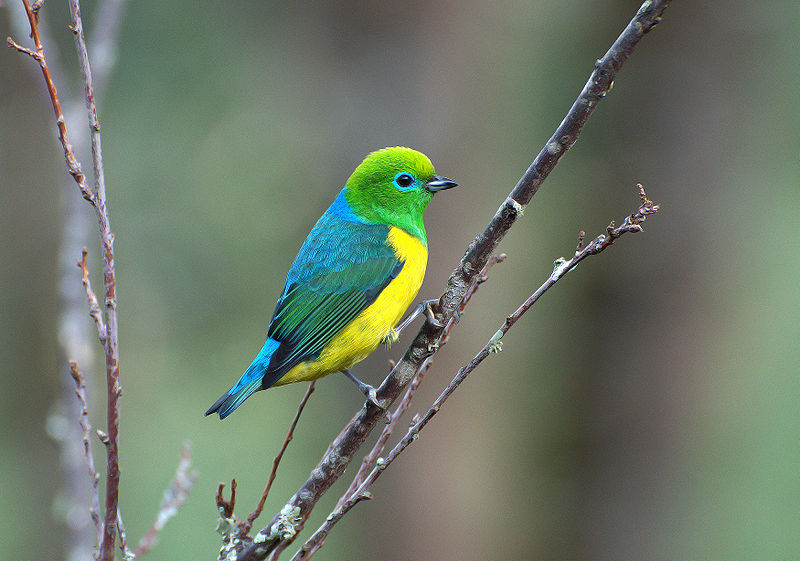
\includegraphics[scale=0.5]{figuras/abntex2-modelo-livro-bandeirinha.jpg}
\fonte{Autoria própria.}
\end{figure}

\begin{quadro}[!htb]
\IBGEtab{%
\caption{Um exemplo de inserção de quadros.}%
\label{exquadro}
}{%
\renewcommand{\arraystretch}{2}
\begin{tabular}{|c|c|c|c|c|c|c|c|c|c|c|c|}
\hline
Atividade & Jan & Fev & Mar & Abr & Mai & Jun & Jul & Ago & Set & Out & Nov \\
\hline
Nome da atividade 01 & X & X & X & X &  &  &  &  &  &  & \\
\hline 
Nome da atividade 02 &  &  &  &  & X & X & X & X & X &  & \\
\hline 
Nome da atividade 03 &  &  &  &  &  &  &  & X & X & X & \\
\hline
Nome da atividade 04 &  &  &  &  &  &  &  &  & X & X & X \\
\hline
Nome da atividade 05 &  &  &  &  &  &  &  &  &  & X & X \\
\hline
\end{tabular}%
}{%
\fonte{Autoria própria.}%
%\nota{Esta é uma nota, que diz que os dados são baseados na regressão linear.}%
%\nota[Anotações]{Uma anotação adicional, que pode ser seguida de várias outras.}%
}
\end{quadro}

\newpage
\begin{scriptsize}
\estiloCodigo
\begin{lstlisting}[caption={Um exemplo de inserção de códigos.}, label=excodigo, captionpos=t]
    em.getTransaction().begin();
        String sql = "select c from Cliente c where c.cpf = :doc ";
        TypedQuery<Cliente> clientes = em.createQuery(sql, Cliente.class);
        clientes.setParameter("doc", cpf);
        em.getTransaction().commit();
        if (!clientes.getResultList().isEmpty()) {
            cli = clientes.getSingleResult();
        } else {
                cli = null;
        }  
    }
\end{lstlisting}
\fonte{Autoria própria.}
\end{scriptsize}

Outra coisa que será bastante necessária, especialmente neste capítulo, é o uso das citações. Basicamente, há três possibilidades de citação: a citação direta curta, a citação direta longa e a citação indireta. Veja alguns exemplos simples:

Para a citação direta curta, coloque o texto de no máximo 3 linhas entre aspas e, no final da sentença, use o comando \cite[s.n]{abntex2-wiki-como-customizar}.

Para a citação indireta, antes de colocar a ideia do(a) autor(a) com suas palavras dentro do seu trabalho, use o comando \citeonline{abntex2-wiki-como-customizar}.

Para a citação direta longa, use o comando
\begin{citacao}
Texto de citação direta longa, seguido da fonte com a indicação da página de onde aquele trecho foi retirado. \cite[p. 2]{abntex2-wiki-como-customizar}
\end{citacao}





\chapter{Materiais e métodos}
\label{metodologia}

Neste capítulo o(a) leitor(a) espera conhecer mais sobre os instrumentos metodológicos e ferramentas que você pretende utilizar para alcançar seus objetivos descritos no Capítulo~\ref{introducao}. Descreva o escopo dos materiais, métodos, técnicas e ferramentas tecnológicas que você irá utilizar. Quando for escrever pense que alguém pode querer reproduzir seu trabalho, portanto, tudo deve ser bem descrito.

\section{Outro exemplo de seção}

Você também pode usar o recursos de seções aqui.

\chapter{Cronograma}
\label{cronograma}

Com o intuito de otimizar a utilização do tempo disponível para a integração desse projeto, fez-se necessária a elaboração de um plano de trabalho, no qual os processos de desenvolvimento do jogo educativo e escrita científica foram decompostos em atividades específicas com prazos de conclusão bem definidos. O cronograma apresentado na Tabela 1 descreve cada atividade e seus respectivos prazos de execução. 

\begin{table}[!htb]
	\IBGEtab{%
		\caption{Cronograma de atividades do Trabalho de Conclusão de Curso}%
		\label{extabela}
	}{%
		\renewcommand{\arraystretch}{2}
		\begin{tabular}{cccccccccccc}
			\hline
			Atividade & Mai & Jun & Jul & Ago & Set & Out & Nov & Dez & Jan & Fev\\
			\hline 
			Definição do Tema & X & &  &  &  &  &  &  &  & \\
			\hline 
			Leitura e Fichamento & X & X & X &  &  &  &  &  &  &\\
			\hline
			Elaboração do Cronograma &  &  & X &  &  &  &  &  &  & \\
			\hline 
			Escrita da Introdução &  &  & X &  &  &  &  &  &  &\\
			\hline
			Escrita do Referencial Teórico &  &  &  & X &  &  &  &  &  &\\
			\hline
			Escrita da Metodologia &  &  &  & X &  &  &  &  &  &\\
			\hline
			Escrita dos Resultados Esperados &  &  &  & X &  &  &  &  &  &\\
			\hline
			Escrita do Resumo &  &  &  &  & X &  &  &  &  &\\
			\hline
			Apresentação do Projeto &  &  &  &  & X &  &  &  &  &\\
			\hline
			Escrita das situações-problema &  &  &  &  & X & X & X &  &  &\\
			\hline
			Escrita da narrativa &  &  &  &  & X & X & X &  &  &\\
			\hline
			Desenvolvimento do jogo &  &  &  &  & X & X & X &  &  &\\
			\hline
			Testes e ajustes do jogo &  &  &  &  &  &  & X & X &  &\\
			\hline
			Implementação do jogo &  &  &  &  &  &  &  & X &  &\\
			\hline
			Avaliação da eficácia do jogo &  &  &  &  &  &  &  & X &  &\\
			\hline
			Escrita dos Resultados e Discussão &  &  &  &  &  &  &  &  & X &\\
			\hline
			Escrita da Conclusão e Resumo &  &  &  &  &  &  &  &  & X &\\
			\hline
			Revisão final &  &  &  &  &  &  &  &  & X &\\
			\hline
			Defesa da monografia &  &  &  &  &  &  &  &  &  & X\\
			\hline
		\end{tabular}%
	}{%
		\fonte{Autoria própria.}
	}
\end{table}


%\chapter{Resultados e discussões}
\label{resultados}

Neste capítulo o(a) leitor(a) espera conhecer os resultados que você obteve durante seu trabalho. Porém, não é "só" isso. Os leitores também querem entender como seus resultados estão interligados com o conhecimento já construído e que foi apresentado por você no Capítulo~\ref{fundamentacao}. Portanto, \textbf{apresente} os resultados e \textbf{discuta-os}, fazendo paralelos com os resultados e as conclusões de outros autores que tratam do mesmo assunto que você está trabalhando.

\section{Mais um exemplo de seção}

Aqui você também pode usar esse recurso se quiser.



%\chapter{Considerações finais}
\label{conclusoes}

Neste capítulo o(a) leitor(a) espera conhecer quais foram as conclusões (ou considerações finais) que você tirou depois de desenvolver seu trabalho, coletar os dados e analisá-los. Você pode fazer uma síntese dos resultados principais, apresentar as limitações do seu trabalho e apresentar propostas de trabalhos futuros para ampliação e melhoria do conhecimento desenvolvido durante seus esforços.

% ---
% Finaliza a parte no bookmark do PDF
% para que se inicie o bookmark na raiz
% e adiciona espaço de parte no Sumário
% ---
\phantompart

% ----------------------------------------------------------
% ELEMENTOS PÓS-TEXTUAIS
% ----------------------------------------------------------
\postextual

% ---
% Referências bibliográficas
% ---
\bibliography{referencias/referencias}

% ---
% Glossário
% ---
%\glossary

% ---
% Apêndices
% ---
\begin{apendicesenv}
% Imprime uma página indicando o início dos apêndices
\partapendices
\chapter{Título do apêndice}

\lipsum[50]

% ---
\chapter{Título do apêndice}

\lipsum[55-57]
\end{apendicesenv}

% ---
% Anexos
% ---
\begin{anexosenv}
% Imprime uma página indicando o início dos anexos
\partanexos
\chapter{Título do anexo}

\lipsum[30]

% ---
\chapter{Título do anexo}


\lipsum[31]


\end{anexosenv}

%---
% INDICE REMISSIVO
%---
\phantompart
\printindex

\end{document}
